\documentclass[tikz, margin=10mm]{standalone}

\usepackage{tikz}
\usetikzlibrary{calc}
\usetikzlibrary{patterns}
\usetikzlibrary{decorations.pathmorphing}

\newdimen\ballradius
\setlength{\ballradius}{5mm}

\newdimen\linewidthofball
\linewidthofball=.6mm

\def\highlightarcfirstangle{-79}
\def\highlightarclastangle{-11}

\newdimen\highlightarcradius
\setlength{\highlightarcradius}{.7\ballradius}

%arguments are x and y where arc begins
\newcommand{\drawHighlight}[2]
{
   \newdimen\linewidthofhighlightarc
   \linewidthofhighlightarc=.5mm
   \draw[ line width=\linewidthofhighlightarc, color=black ]
      (\dimexpr #1\relax, \dimexpr #2\relax)
         arc ( \highlightarcfirstangle:\highlightarclastangle:\highlightarcradius ) ;
}

%arguments are coordinates x and y where to draw
\newcommand{\drawBall}[2]
{
   \draw[ line width=0.1pt, color=white, fill=white ] (\dimexpr #1\relax, \dimexpr #2 \relax) circle (\ballradius) ;
   \draw[ line width=\dimexpr \linewidthofball\relax, color=black ] (\dimexpr #1\relax, \dimexpr #2 \relax) circle (\ballradius) ;

   %the center of "(x,y) arc (f:g:r)" is at point (x-r*cos(f), y-r*sin(f))
   \pgfmathsetmacro{\arcshiftcos}{cos(\highlightarcfirstangle)}
   \pgfmathsetmacro{\arcshiftsin}{sin(\highlightarcfirstangle)}
   \newdimen\arcbeginx
   \newdimen\arcbeginy
   \setlength{\arcbeginx}{\arcshiftcos\highlightarcradius}
   \setlength{\arcbeginy}{\arcshiftsin\highlightarcradius}
   \addtolength{\arcbeginx}{#1}
   \addtolength{\arcbeginy}{#2}

   \drawHighlight{\arcbeginx}{\arcbeginy}
}

% gluon decoration, based on the original coil decoration
% https://tex.stackexchange.com/questions/64786/coil-path-decoration-without-straight-segment

\makeatletter

\pgfdeclaredecoration{gluon}{coil}
{
  \state{coil}[switch if less than=%
    0.5\pgfdecorationsegmentlength+%>
    \pgfdecorationsegmentaspect\pgfdecorationsegmentamplitude+%
    \pgfdecorationsegmentaspect\pgfdecorationsegmentamplitude to last,
               width=+\pgfdecorationsegmentlength]
  {
    \pgfpathcurveto
    {\pgfpoint@oncoil{0    }{ 0.555}{1}}
    {\pgfpoint@oncoil{0.445}{ 1    }{2}}
    {\pgfpoint@oncoil{1    }{ 1    }{3}}
    \pgfpathcurveto
    {\pgfpoint@oncoil{1.555}{ 1    }{4}}
    {\pgfpoint@oncoil{2    }{ 0.555}{5}}
    {\pgfpoint@oncoil{2    }{ 0    }{6}}
    \pgfpathcurveto
    {\pgfpoint@oncoil{2    }{-0.555}{7}}
    {\pgfpoint@oncoil{1.555}{-1    }{8}}
    {\pgfpoint@oncoil{1    }{-1    }{9}}
    \pgfpathcurveto
    {\pgfpoint@oncoil{0.445}{-1    }{10}}
    {\pgfpoint@oncoil{0    }{-0.555}{11}}
    {\pgfpoint@oncoil{0    }{ 0    }{12}}
  }
  \state{last}[next state=final]
  {
    \pgfpathcurveto
    {\pgfpoint@oncoil{0    }{ 0.555}{1}}
    {\pgfpoint@oncoil{0.445}{ 1    }{2}}
    {\pgfpoint@oncoil{1    }{ 1    }{3}}
    \pgfpathcurveto
    {\pgfpoint@oncoil{1.555}{ 1    }{4}}
    {\pgfpoint@oncoil{2    }{ 0.555}{5}}
    {\pgfpoint@oncoil{2    }{ 0    }{6}}
  }
  \state{final}{}
}

\def\pgfpoint@oncoil#1#2#3{%
  \pgf@x=#1\pgfdecorationsegmentamplitude%
  \pgf@x=\pgfdecorationsegmentaspect\pgf@x%
  \pgf@y=#2\pgfdecorationsegmentamplitude%
  \pgf@xa=0.083333333333\pgfdecorationsegmentlength%
  \advance\pgf@x by#3\pgf@xa%
}

\makeatother

%arguments
%  #1 and #2 are x and y of first ball's center point,
%  #3 and #4 are x and y of second ball's center point
\newcommand\drawSpring[4]
{
   \def\springaspect{0.5}

   \newdimen\springamplitude
   \springamplitude=2mm

   \newdimen\segmentadvance
   \segmentadvance=2.3mm

   \newdimen\linewidthofspring
   \linewidthofspring=\linewidthofball

   \draw[ color=black,
          line width=\dimexpr \linewidthofspring\relax,
          decoration={ aspect=\springaspect,
                       segment length=\dimexpr \segmentadvance\relax,
                       amplitude=\dimexpr \springamplitude\relax,
                       gluon },decorate ]
      (\dimexpr #1\relax, \dimexpr #2\relax) -- (\dimexpr #3\relax, \dimexpr #4\relax) ;
}

\begin{document}

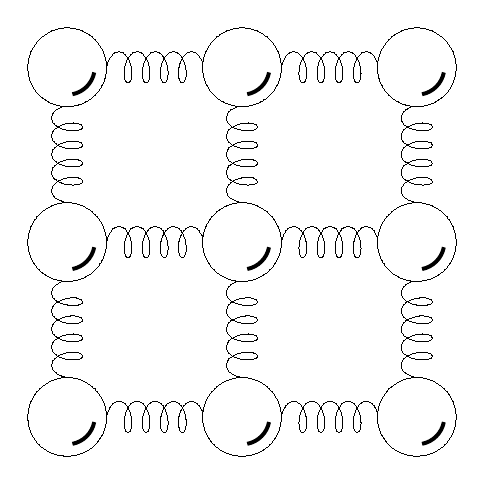
\begin{tikzpicture}

  \newdimen\ballxstep
  \newdimen\ballystep
  \setlength{\ballxstep}{4.44\ballradius}
  \setlength{\ballystep}{4.44\ballradius}

  \newdimen\yforspring
  \yforspring=\ballystep
  \addtolength{\yforspring}{-\ballradius}

  \newdimen\xforspring
  \xforspring=\ballxstep
  \addtolength{\xforspring}{-\ballradius}

  \newdimen\theZero
  \theZero=0mm

  \newdimen\forspringatzero
  \forspringatzero=\theZero
  \addtolength{\forspringatzero}{\ballradius}

  \drawSpring{\theZero}{\forspringatzero}{\theZero}{\yforspring}
  \drawSpring{\theZero}{-\yforspring}{\theZero}{-\forspringatzero}
  \drawSpring{\forspringatzero}{\theZero}{\xforspring}{\theZero}
  \drawSpring{-\xforspring}{\theZero}{-\forspringatzero}{\theZero}
%
  \drawSpring{-\ballxstep}{-\yforspring}{-\ballxstep}{-\forspringatzero}
  \drawSpring{-\ballxstep}{\forspringatzero}{-\ballxstep}{\yforspring}
  \drawSpring{\ballxstep}{\forspringatzero}{\ballxstep}{\yforspring}
  \drawSpring{\ballxstep}{-\yforspring}{\ballxstep}{-\forspringatzero}
%
  \drawSpring{\forspringatzero}{\ballystep}{\xforspring}{\ballystep}
  \drawSpring{-\xforspring}{\ballystep}{-\forspringatzero}{\ballystep}
  \drawSpring{\forspringatzero}{-\ballystep}{\xforspring}{-\ballystep}
  \drawSpring{-\xforspring}{-\ballystep}{-\forspringatzero}{-\ballystep}

  \drawBall{-\ballxstep}{\ballystep}
  \drawBall{\theZero}{\ballystep}
  \drawBall{\ballxstep}{\ballystep}
  \drawBall{-\ballxstep}{\theZero}
  \drawBall{\theZero}{\theZero}
  \drawBall{\ballxstep}{\theZero}
  \drawBall{-\ballxstep}{-\ballystep}
  \drawBall{\theZero}{-\ballystep}
  \drawBall{\ballxstep}{-\ballystep}

\end{tikzpicture}

\end{document}

